\subsection{Bewertung des Sprints}
Im zweiten Sprint wurde ein Aspekt der Anwendung überarbeitet und es sind weiter Features dazugekommen. Bei dem überarbeiteten Feature handelt es sich um die Monsterliste. Hinzugekommen ist das Bonusfeature, welches das Bearbeiten der Steuerung durch den Nutzer ermöglichen soll. Des Weiteren wurde das komplette Kampfgeschehen implementiert, sodass alle Kampfsituationen durchgeführt und angezeigt werden können.  Zusätzlich gab es einige technische Anforderungen, die sichergestellt werden mussten. Die Internationalisierung ist ein Bonusfeature aus der zweiten Veröffentlichung und musste ebenfalls sichergestellt werden.\\
\begin{figure}[H]
    \center
    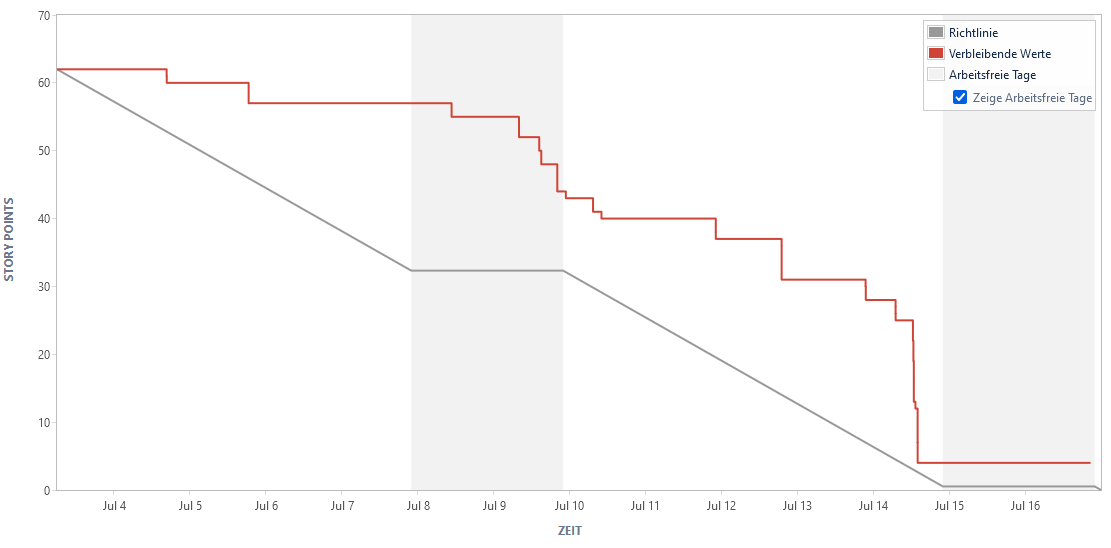
\includegraphics[height=0.5\textwidth]{images/burndown/sprint2Story.png}
    \caption{Burndown-Diagramm: Release 3: Sprint 2 Story Points}
    \label{fig: sprint2Story}
\end{figure}

Wie schon im ersten Sprint wurden im zweiten Sprint ebenfalls nicht alle Storys abgeschlossen. Wie in der Abbildung \ref{fig: sprint2Story} zu sehen ist, hängt dies mit zwei Phasen des Sprints zusammen. So wurde bis zum Wochenende der ersten Woche nicht sehr viele Storys abgearbeitet. Am Wochenende ist dann zwar ein guter Fortschritt erzielt worden, der Rückstand konnte aber nicht komplett aufgeholt werden. Auch zu Beginn der zweiten Woche gab es wieder wenig Fortschritt, was die zweite schlechte Phase darstellt. Zwar wurde am Freitag versucht, alle Anforderungen zu implementieren, aber der Rückstand war zu groß. Dabei sind zwei Storys und ein Bug nicht abgeschlossen worden. Die Storys \hyperlink{S236}{STP23M-236} und \hyperlink{S277}{STP23M-277} wurden aufgrund von Zeitmangel am Freitag nicht mehr fertiggestellt. Für den Bug \hyperlink{S432}{STP23M-432} wurde keine Lösung gefunden. \\ Die Bewertung kann, aufgrund der nicht abgeschlossenen Vorgänge, nicht positiv ausfallen. So müssen und werden die fehlenden Anforderungen in der vierten Veröffentlichung nachgereicht. Auch die geforderten 70\% Test Coverage wurde mit 64.17\% nicht erreicht. Auch diese wird in der vierten Veröffentlichung verbessert werden müssen.

\subsubsection{Erhöhung der Vorgänge}
Im zweiten Sprint der dritten Veröffentlichung gab es fünf Umfangsänderungen.
\begin{figure}[H]
    \center
    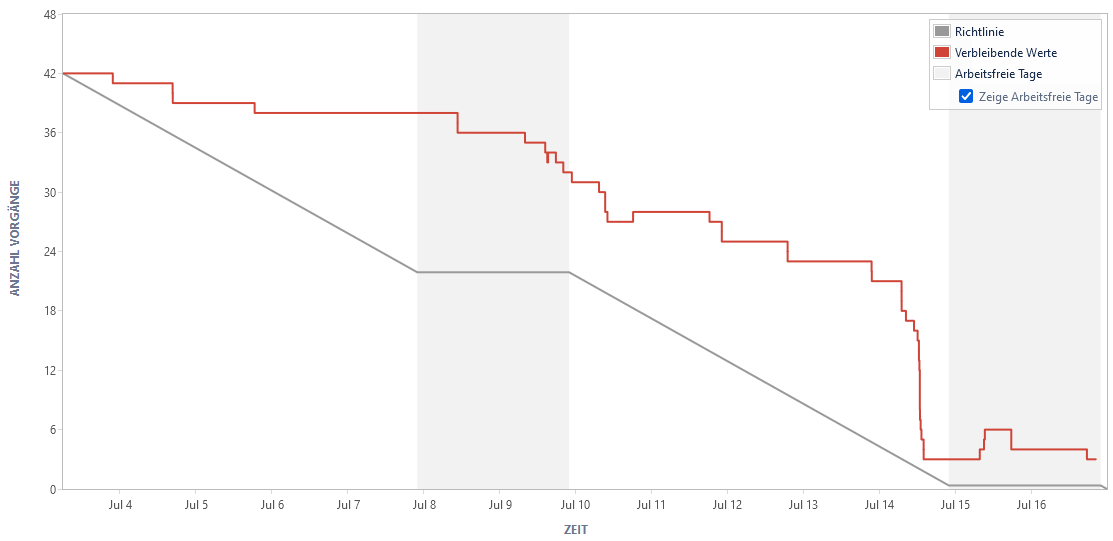
\includegraphics[height=0.5\textwidth]{images/burndown/sprint2vorg.png}
    \caption{Burndown-Diagramm: Release 3: Sprint 2 Vorgänge}
    \label{fig: sprint2vorg}
\end{figure}

In der ersten Woche des Sprints ist der Bug \hyperlink{S439}{STP23M-439} hinzugekommen. Dieser wurde schnell bearbeitet. In der zweiten Woche vor der Veröffentlichung am Freitag ist der Bug \hyperlink{S438}{STP23M-438} dazugekommen, der nicht direkt bearbeitet wurde. Am Wochenende nach der Veröffentlichung sind mit \hyperlink{S478}{STP23M-478}, \hyperlink{S479}{STP23M-479} und \hyperlink{S480}{STP23M-480} drei weitere Bugs dazugekommen. Die letzten beiden wurden schnell abgearbeitet. Lediglich \hyperlink{S478}{STP23M-478} wurde erst am Sonntag geschlossen.

\subsubsection{Zeitschätzung}
Die Zeitschätzung für alle Vorgänge des zweiten Sprints betrug 91 Stunden und 40 Minuten. Die tatsächliche benötigte Zeit betrug jedoch 94 Stunden und 35 Minuten. Die Abweichung beträgt demnach nur circa drei Stunden, was im Vergleich zum ersten Sprint mit circa 15 Stunden zunächst positiv erscheint. Allerdings wurden, wie oben beschreiben, die Storys \hyperlink{S236}{STP23M-236} und \hyperlink{S277}{STP23M-277} und der Bug \hyperlink{S432}{STP23M-432} nicht abgeschlossen, wodurch hier keine positive Bewertung gegeben werden kann. 